\documentclass[10pt, conference]{IEEEtran}
\IEEEoverridecommandlockouts
% The preceding line is only needed to identify funding in the first footnote. If that is unneeded, please comment it out.
\usepackage{cite}
\usepackage{caption}
\usepackage{amsmath,amssymb,amsfonts}
\usepackage{algorithmic}
\usepackage{graphicx}
\usepackage{textcomp}
\usepackage{listings}
\usepackage{xcolor}
\def\BibTeX{{\rm B\kern-.05em{\sc i\kern-.025em b}\kern-.08em
    T\kern-.1667em\lower.7ex\hbox{E}\kern-.125emX}}
\begin{document}

%%%%%%%%%%%%%%%%%%%%%%%%%%%%%%%%%%%%%%%%%%%%%%%%%%%%%%%%%%%%%%%%%%%%%%%%%%%%%%%%%%%%%%%%%

\title{MidcurveLLM: Geometric Dimension Reduction using Large Language Models}

\author{\IEEEauthorblockN{Yogesh Kulkarni}
\IEEEauthorblockA{ yogeshkulkarni@yahoo.com http://orcid.org/0000-0001-5431-5727}
}

\maketitle

\begin{abstract}
Lower-dimensional representations of shapes are essential for numerous applications. The midcurve, a one-dimensional (1D) representation of a two-dimensional (2D) planar shape, serves as a concise and informative descriptor. Widely utilized in animation, shape matching, retrieval, finite element analysis, and other fields, midcurves offer a compact means of capturing geometric information.

This paper delves into the usage of Large Language Models (LLMs) for computing midcurves of 2D geometric profiles. Traditional methods face challenges with intricately shaped profiles, prompting a thorough evaluation of LLMs' efficacy. The research frames midcurve extraction as a Graph Summarization problem, addressing specific challenges in geometric representation, variable-length inputs, and branched midcurves. Neural network-based approaches, such as Sequence-to-Sequence and Image-to-Image models, are also presented, with Text-to-Text transformation using LLMs being explored as a novel and potentially effective approach. 
\end{abstract}



% \begin{abstract}
% Lower-dimensional representations of shapes are essential for numerous applications. The midcurve, a one-dimensional (1D) representation of a two-dimensional (2D) planar shape, serves as a concise and informative descriptor. Widely utilized in animation, shape matching, retrieval, finite element analysis, and other fields, midcurves offer a compact means of capturing geometric information. This paper explores diverse methods for midcurve computation, considering various input shape types (e.g., images, sketches) and processing techniques (thinning, Medial Axis Transform (MAT), Chordal Axis Transform (CAT), Straight Skeletons).


% This paper further investigates the integration of Large Language Models (LLMs) for computing midcurves in 2D geometric profiles. LLMs offer a promising avenue for distilling complex shapes while retaining key geometric details. Notably, traditional methods like Medial Axis Transform and Chordal Axis Transform often encounter difficulties with intricately shaped profiles and diverse connections, prompting a thorough evaluation of LLMs' potential efficacy in this domain.
% This research tackles the challenge of midcurve extraction from 2D geometric profiles, framing it as a Graph Summarization problem analogous to text summarization. It meticulously addresses the specific challenges inherent in this domain, including geometric representation, variable-length input profiles, and branched midcurves. It explores neural network-based approaches such as Sequence-to-Sequence and Image-to-Image models, highlighting their strengths and limitations. Promisingly, Text-to-Text transformation using Large Language Models (LLMs) emerges as a novel and effective approach, demonstrated through prompt-based evaluations. This study contributes significantly to the advancement of midcurve computation, paving the way for efficient and accurate representation of complex 2D shapes.


% Fine-tuning LLMs using a Boundary Representation (Brep) structure demonstrates potential for overcoming the limitations inherent in sequential point lists. However, challenges remain in LLM fine-tuning, ranging from model quality to dataset size, demanding further investigation and refinement. The complex nature of midcurve generation necessitates ongoing exploration, particularly in conjunction with the evolving capabilities of LLMs. This research opens exciting avenues for scholars and practitioners to delve deeper into the realm of geometric dimension reduction using LLMs, paving the way for significant advancements in shape analysis and representation. 
% \end{abstract}

\begin{IEEEkeywords}
midcurve, generative ai, large language models, graph algorithms, neural networks
\end{IEEEkeywords}

\section{Introduction}
\label{sec:1}
In the field of Computer-Aided Design (CAD), especially concerning thin-walled solids such as sheet metal and plastic components, the process of dimensional reduction is pivotal for accelerating Computer-Aided Engineering (CAE) analysis. This acceleration is realized by generating Mid-surfaces, which are surfaces positioned equidistantly between the bounding surfaces of the original solid. These Mid-surfaces function as highly effective substitutes for analysis, leading to a notable decrease in computational complexity. Despite their significance, the generation of Mid-surfaces continues to be a labor-intensive and mostly manual task due to the limited availability of robust and efficient automated methodologies.\cite{medial2010}.


Automated methods currently employed in Mid-surface generation often face challenges, resulting in undesirable artifacts like gaps, absent patches, and overlapping surfaces. Rectifying these errors manually is a highly time-consuming endeavor, demanding hours or even days of meticulous effort. This underscores the pressing necessity for a dependable and streamlined automated procedure to produce precise and resilient Mid-surfaces.

The notion of Mid-surfaces extends to planar shapes in the realm of two-dimensional (2D) geometry, where its counterpart is referred to as the Midcurve. Described as a curve equidistant from the bounding curves of a 2D profile, the Midcurve offers a simplified representation while preserving essential geometric details (Fig. \ref{fig_medialmethods}). Despite the existence of several conventional methods for Midcurve computation, the persistent challenge lies in accurately representing intricate shapes with diverse connections.

    \begin{center}
	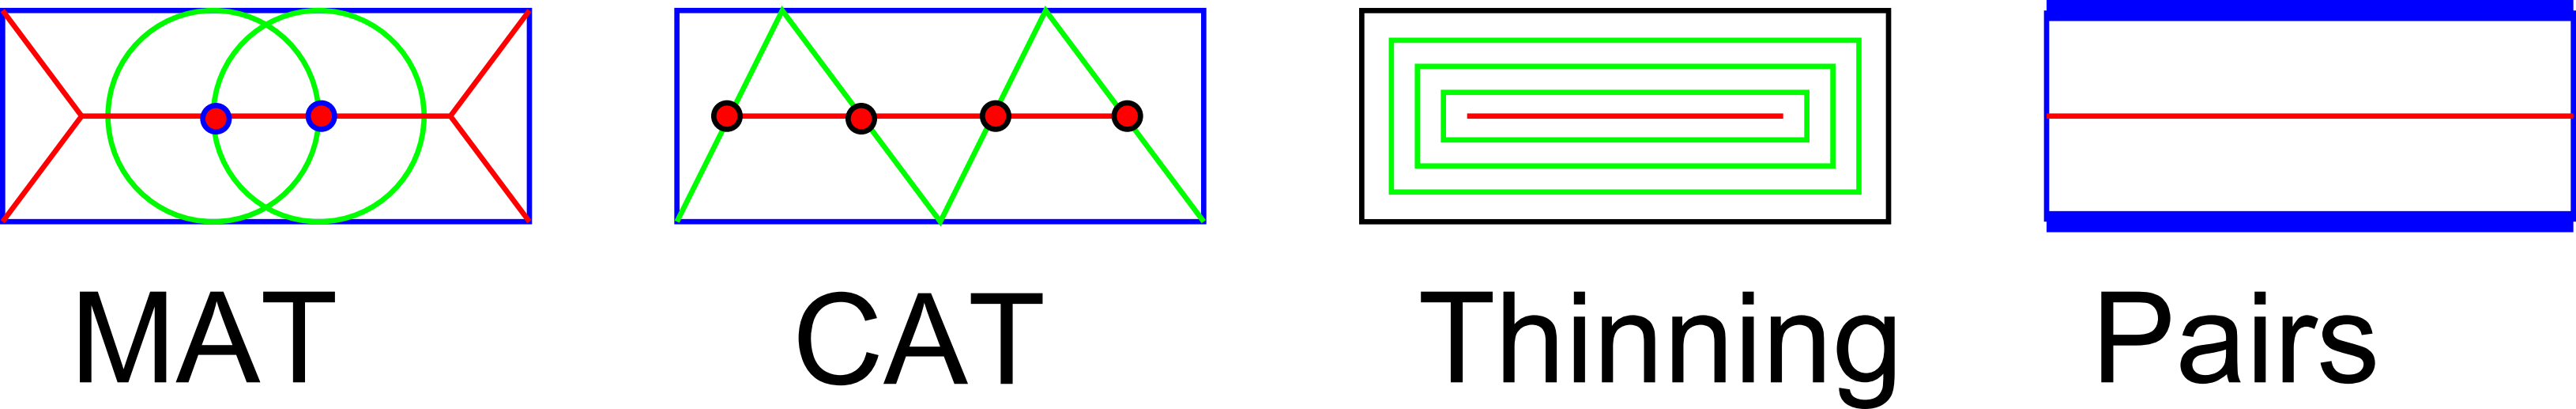
\includegraphics[width=\linewidth]{images/MedialMethodsOnlyShort}
	\captionof{figure}{Medial Object computation methods} \cite{midcurvenn2022}
	\label{fig_medialmethods}
    \end{center}
	
%Figure \ref{fig_letters} shows some of the input shapes which can be considered. English alphabets are chosen for easy understanding and verification of the proposed method.
%
%     \begin{center}
%	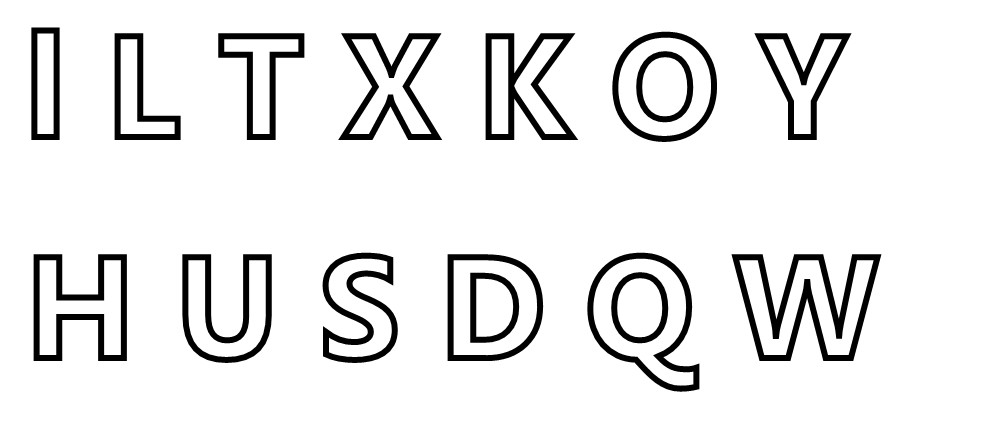
\includegraphics[width=0.8\linewidth]{images/Letters}
%	\captionof{figure}{2D Thin Polygonal shapes} \cite{midcurvenn2023}
%	\label{fig_letters}
%    \end{center}
	
The research initiative MidcurveNN \cite{midcurvenngithub} explores the feasibility of utilizing Neural Networks, with a current emphasis on Large Language Models (LLMs), to address the complex task of Midcurve generation.

% LLMs offer a powerful and versatile tool for processing complex information, and their potential to revolutionize the field of Midcurve computation is being thoroughly explored within this research framework. We aim to address the limitations of existing methods and establish a robust and efficient workflow for generating accurate and reliable Midcurves for diverse 2D geometric profiles.

%Traditional methods often encounter limitations when faced with complex shapes and diverse connections. LLMs, on the other hand, offer a unique opportunity to overcome these limitations due to their ability to process and analyze large amounts of data, including complex geometric representations. By leveraging the power of LLMs, MidcurveNN aims to establish a robust and efficient framework for automatic midcurve generation, paving the way for significant advancements in shape analysis and representation.

\section{Related Work}
\label{sec:2}

The quest for efficient and robust methods for computing Mid-surfaces and Midcurves has spanned several decades, with significant advancements documented in a comprehensive review of the field available in the survey paper \cite{medial2010} and also show in Fig. \ref{fig_timeline}.

     \begin{center}
	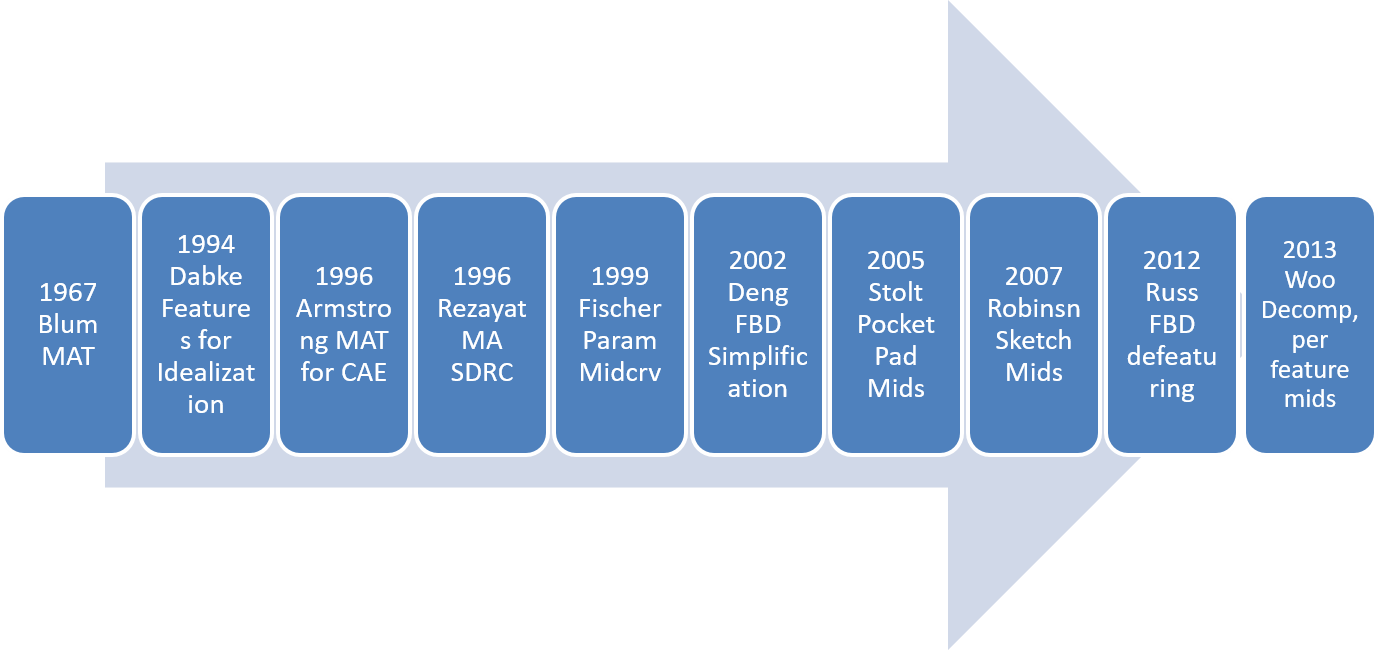
\includegraphics[width=0.8\linewidth]{images/midcurve15}
	\captionof{figure}{Midcurve Research Timeline}
	\label{fig_timeline}
    \end{center}
    

\subsection{Classical Approaches}
\label{subsec:1}
Several key observations emerge from the analysis of classical approaches:
\begin{itemize}
\item {\bf Formal methods}: Approaches like Medial Axis Transform (MAT) while versatile and reversible for shapes of varying thickness, face drawbacks such as generating superfluous branches, diminishing shape size, and sensitivity to base geometry changes. MAT-based methods may incur computational expenses and necessitate re-computation with altered base geometries, introducing the possibility of divergent outcomes.
\item {\bf Heuristic methods}: Chordal Axis Transform (CAT) approaches demand pre-existing meshes, posing challenges for complex 2D profiles, while Thinning approaches, reliant on straight line skeleton split events, may yield counter intuitive results, especially at sharp reflex vertices. The Pairs approach encounters difficulties in preserving continuity with non-one-to-one input forms, and Midcurve by profile decomposition, though less embraced, grapples with generating redundant sub-shapes, rendering it ineffective and unstable for further processing.
\end{itemize}

The author's own prior work (Fig. \ref{fig_phd})  demonstrates success on simpler shapes, it suffers from scalability limitations due to its rule-based nature.

     \begin{center}
	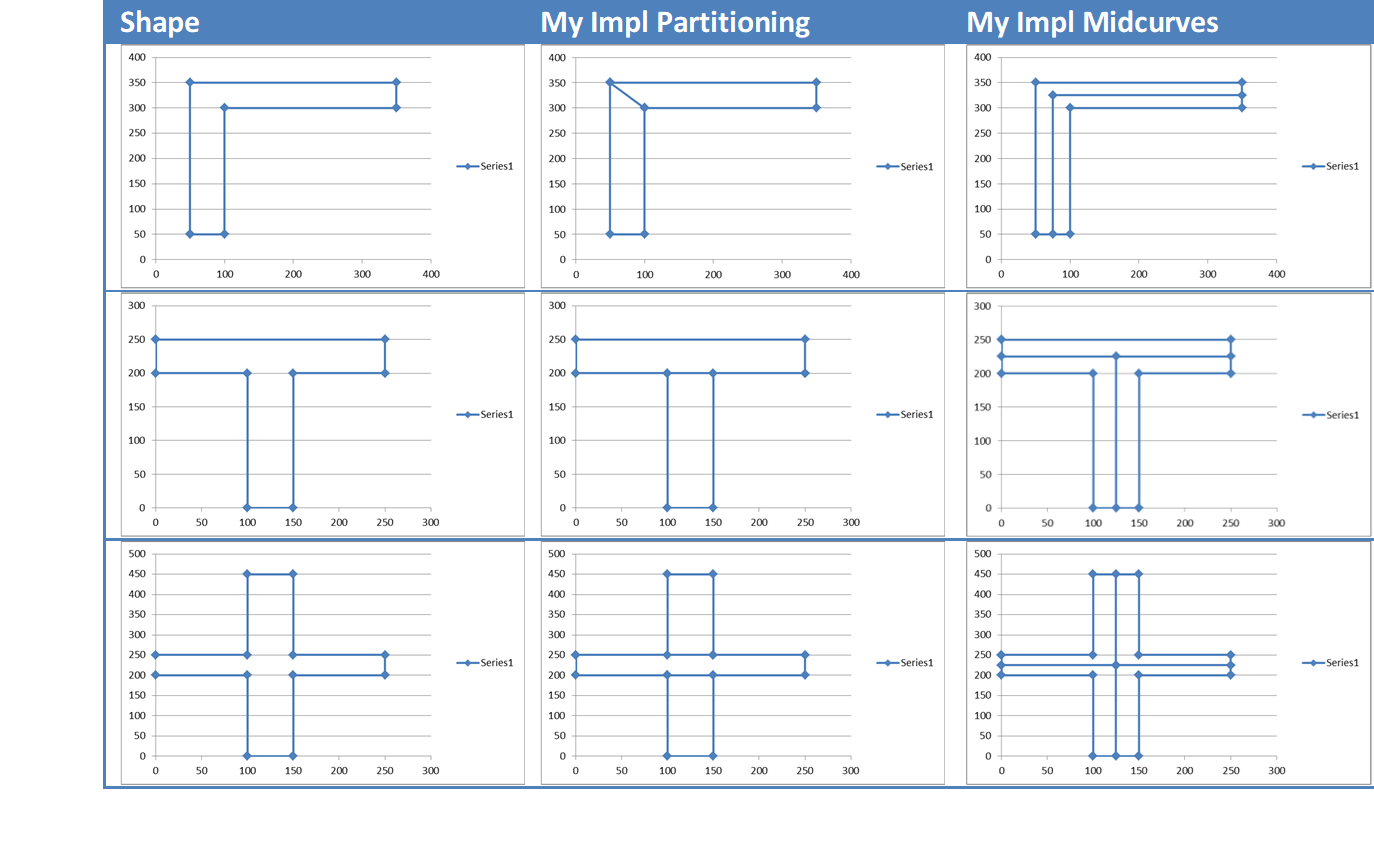
\includegraphics[width=\linewidth]{images/midcurve16}
	\captionof{figure}{Midcurve using Cellular Decomposition} \cite{kulkarni2017}
	\label{fig_phd}
    \end{center}


\subsection{Recent Advances and Research Gaps}
\label{subsec:2}

Recent advancements have seen the integration of Neural Network-based techniques for Skeleton Midcurve computation, primarily through image processing. Notable examples include:
\begin{itemize}
\item Rodas, Neumann, and Wimmer 2020\cite{Rodas2019JointOB}: Employed Deep Convolutional Neural Networks to simultaneously compute object boundaries and skeletons.
\item Shen, Zhou, and Zeng 2021 \cite{shen2021convolutional}: Developed a Convolutional neural network-based skeleton extractor capturing both local and non-local image context.
\item Shen et al 2021 \cite{shen2016object}: Introduced a hierarchical feature learning mechanism for skeleton extraction.
\item Wang et al. 2023 \cite{wang2018deepflux}: Focused on content flux in skeletons as a learning objective.
\item Panichev \cite{Panichev_2019_CVPR_Workshops}: Utilized U-net to extract skeletons, although not for Midcurve generation.
\end{itemize}

Despite these advancements, a review of the state-of-the-art emphasizes the need for Midcurve computation approaches that consider several key factors:
\begin{itemize}
\item {\bf Application context}: The choice of method should be guided by the specific application and the desired level of accuracy.
\item {\bf Shape characteristics}: Different approaches may be better suited for specific types of shapes, such as primitive-shaped, thin sub-polygons.
\item {\bf Aspect ratio}: The aspect ratio of sub-polygons can significantly impact the effectiveness of various methods.
\end{itemize}
The current research gap lies in the need for efficient and accurate Midcurve generation for primitive-shaped, thin sub-polygons. Existing methods often struggle with non-primitive, skewed shapes and may yield inappropriate Midcurves


\section{Proposed Method}
\label{sec:3}

Computation of midcurve, in its original form, is transformation of a 2D thin closed, with/without-holes polygon to 1D open/closed/branched polyline. Research shown in \cite{dimred2017} details one of the effective midcurve computation techniques, based on rule-based computational geometry approach. Such techniques have a shortcoming of not being scalable or generic enough to be able to handle variety of shapes. Deep Learning neural network architectures have  shown potential of developing such generic models. This dimension reduction transformation is modeled as Sequence to Sequence (Seq2Seq) neural architecture, like Machine Translation.

In the current problem, the input and the output sizes could be different not just in a single sample, but across all samples. Many current Seq2Seq neural networks need fixed size inputs and outputs, which if not present in data, are artificially managed by adding padding of certain improbable value. Such padding is not appropriate for the current midcurve computation problem, as the padding-value can inappropriately get treated as part of the valid input. In this initial phase, to circumvent the problem of variable size, image-based inputs and outputs are used, which are of fixed size. Both input and output polygonal shapes are rasterized into images of $100 \times 100$, thus making them fixed size for all samples, irrespective of the original shapes.


Research shown in \cite{midcurvenn2022}, \cite{midcurvenn2023} and \cite{Kulkarni2023} use such network for midcurve computation in the form of image-to-image mode. Input images have thin polygonal shapes whereas output images have corresponding midcurve images. Fig. \ref{fig_endecoder} shows the Encoder-decoder architecture idea leveraged for MidcurveNN.

     \begin{center}
	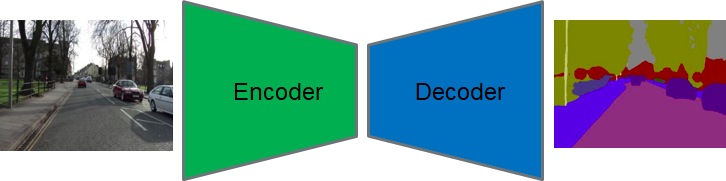
\includegraphics[width=0.8\linewidth]{images/enc-dec}
	\captionof{figure}{Encoder-Decoder Architecture} \cite{DasSeg2019}
	\label{fig_endecoder}
    \end{center}
    
This paper proposes a novel approach to Midcurve generation using Deep Learning, specifically Large Language Models (LLMs). LLMs offer a unique opportunity to leverage their powerful language processing capabilities to learn and represent complex geometric relationships between 2D profiles and their corresponding Midcurves. This approach promises to overcome the limitations of existing methods and offer a robust and efficient solution for Midcurve computation


\subsection{Problem Statement}
\label{subsec:3}

Given a 2D closed shape (simple, convex, closed polygon) represented as a set of points or connected lines, find its corresponding midcurve (polyline, either closed or open).

The midcurve should be generated while preserving the key geometric properties of the original shape, similar to how text summarization retains the essence of a longer text document. This translates to the problem of Graph Summarization/Dimension-Reduction/Compression, where we aim to reduce the complexity of a larger graph (representing the polygon) to a smaller, simplified graph (representing the midcurve) while maintaining its underlying structure.

\subsection{Geometry Representation}
\label{subsec:4}

A fundamental challenge in employing Neural Networks for midcurve generation lies in the inherent differences between geometric shapes and the vector representations required by these models. Traditional encoders and decoders rely on fixed-size input and output vectors, posing difficulties for variable-length geometric shapes like polygons and polylines.

Several key issues prevent modeling shapes as simple sequences:
\begin{itemize}
\item {\bf Non-sequential nature}: While a polygon may appear as a sequence of points, it lacks the inherent order and directionality of true sequential data.
\item {\bf Incomplete representation}: Shapes like Y or concentric circles cannot be drawn without lifting a pencil, violating the fundamental principle of sequence generation.
\item {\bf Spatial information loss}: Converting geometric shapes to vectors leads to information loss, particularly regarding spatial relationships and relative positions.
\end{itemize}

Existing graph-based representations, while addressing connectivity, fall short in capturing the crucial spatial information necessary for accurate midcurve generation. Nodes in such graphs carry coordinates, but the arcs lack inherent geometry (e.g., curvature, line segments). This limits the effectiveness of Graph Neural Networks, which rely on convolution and pooling operations that are not well-suited for handling both topology and geometry.
Therefore, the research requires significant innovation in geometric-graph embedding techniques. Such methods should enable convolution operations at nodes while incorporating the geometry of arcs (e.g., sets of point coordinates). Additionally, a novel pooling strategy needs to be developed to effectively aggregate information from neighboring nodes, arcs, and their respective geometric features into a single, meaningful representation. Addressing these challenges is crucial for enabling Neural Networks to learn and process the complex geometric relationships underlying 2D shapes and their corresponding midcurves.

\subsection{Variable Lengths Issue}
\label{subsec:5}

Midcurve generation presents a unique challenge in the domain of Neural Network-based dimension reduction. Unlike traditional sequence-to-sequence tasks, this problem involves variable-length inputs and outputs. The input sketch profile, which is a 2D parametric representation, can have varying numbers of points and line segments. Similarly, the output midcurve, being a 1D representation, exhibits variable length and may even have branches, deviating from the linear structure expected by standard encoders and decoders.


This variable length characteristic poses significant difficulties for existing deep learning libraries like TensorFlow, which require fixed-size input and output vectors. Padding approaches, commonly employed for handling variable lengths, prove problematic in this scenario. Traditional padding values like "0, 0" would be misconstrued as valid points within the geometric representation of the shape.


Furthermore, the non-linear connections present in both input polygons and branched midcurves render them unsuitable for typical Sequence-to-Sequence (seq2seq) networks. These networks rely on the linear order of data, which is not present in our domain due to potential loops and branches.
To address these challenges, alternative approaches need to be explored. One potential solution involves representing both the input and output using a fixed-size image format like 64x64 pixels. By coloring the profile and midcurve in the corresponding image bitmap, we can leverage the established capabilities of LSTM encoders and decoders for seq2seq processing. This approach allows for data augmentation through shifting, rotating, and scaling both input and output images, further enriching the training data.


However, this approach is limited to 2D sketch profiles with only linear segments and single, simple polygons without holes. The question of vectorization remains crucial. Representing each point as a 2D vector leads to variable-length input and output vectors, posing challenges for training. While potential solutions like padding with "0, 0" or "NULL" values exist, their validity within the context of geometric representations needs further investigation.
Additionally, exploring different network architectures beyond simple feed-forward networks is vital. Recurrent Neural Networks (RNNs) and specifically LSTMs are well-suited for handling sequential data and could offer improved performance. Exploring dedicated architectures designed for graph-based data with variable lengths and non-linear connections could also be a promising avenue.

Addressing the variable length issue is a crucial step in enabling Neural Networks to effectively learn and generate midcurves from diverse 2D shapes. By investigating alternative representations, data augmentation techniques, and specialized network architectures, we can pave the way for robust and accurate midcurve generation using deep learning.


\section{Implementation}
\label{sec:4}

While representing geometric shapes as images addresses both the representation and variable-size issues, it introduces a significant dilution in information accuracy. True geometric shapes are vector-based, whereas images are raster-based. This introduces an inherent approximation, which can potentially affect the quality of the generated midcurve. Additionally, the predicted output from an image-based model likely requires post-processing to convert it back into a geometric form, introducing another layer of complexity and potential errors.
Therefore, this project proposes a three-phase approach to address these challenges:

\begin{itemize}
\item {\bf Phase I}: Image to Image Transformation Learning:
	\begin{itemize}
	\item {\bf Img2Img}: This phase focuses on learning image-to-image transformation using fixed-size 100x100 bitmaps.
	\item {\bf Data Augmentation}: The training data will be augmented by scaling, rotating, and translating both input and output shapes within the fixed size.
	\item {\bf Network Architecture}: An Encoder-Decoder network, specifically Semantic Segmentation or Pix2Pix, will be employed for image-based dimension reduction.
	\end{itemize}
	
\item {\bf Phase II}: Text to Text Transformation Learning:
	\begin{itemize}
	\item {\bf Geometric Representation}: A text-based representation of the geometry/graph/network will be explored to leverage Natural Language Processing (NLP) techniques.
	\item {\bf Existing Methods}: The paper (Fatemi, Halcrow, and Bryan 2023) surveys several text-based representations for graph data, but none appear specifically suited for geometric shapes.
	\item {\bf Proposed Approach}: A geometry representation similar to 2D Boundary Representation (B-rep) will be utilized, adapting the concept from 3D to 2D.
	\end{itemize}
		
\item {\bf Phase III}: Geometry to Geometry Transformation Learning:
	\begin{itemize}
	\item {\bf Graph Representation}: Both input and output polyline graphs will be constructed with $(x,y)$ coordinates as node features and edge information represented by node ID pairs.
	\item {\bf Polyline vs. Curve Representation}: For polylines, edges are straight lines, eliminating the need for storing geometric intermediate points as features. For curves, a fixed number $n$ of sampled points will be stored as features.
	\item {\bf Network Architecture}: An Image-Segmentation-like Encoder-Decoder network will be implemented, incorporating Graph Convolution Layers from DGL in place of the usual 2D convolution layers typically used in image-based models.
	\item {\bf Data Generation}: A variety of input-output polyline pairs will be generated using geometric transformations, avoiding the image-based transformations employed in Phase I.
	\item {\bf Potential Techniques}: The use of Variational Graph Auto-Encoders will be investigated for its potential benefits in this phase.
	\end{itemize}
\end{itemize}		
This phased approach aims to address the challenges of variable-size inputs and outputs while achieving accurate and robust midcurve generation by leveraging appropriate representation techniques and network architectures. Phase I lays the groundwork with a well-established approach in image-based processing, while Phase II explores the potential of text-based representations for geometric information. Phase III ultimately focuses on developing a network capable of directly processing and transforming geometric data, offering the most promising avenue for achieving high-fidelity midcurve generation.

\subsection{Image-to-Image based Approach}
\label{subsec:6}

     \begin{center}
	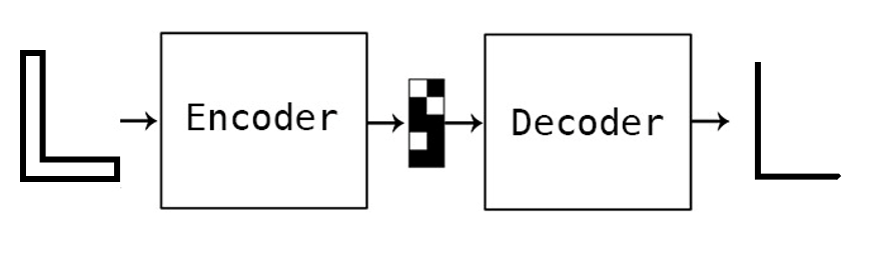
\includegraphics[width=0.8\linewidth]{images/midcurve26}
	\captionof{figure}{Midcurve by Encoder Decoder} \cite{midcurvenn2022}
	\label{fig_ecd}
    \end{center}

Such Transformers taking variable length input and output graphs have not been established. So, would taking this problem to image domain help?

     \begin{center}
	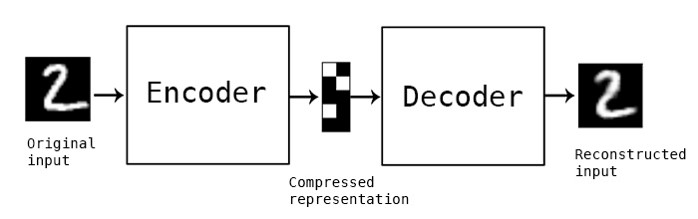
\includegraphics[width=0.8\linewidth]{images/midcurve25}
	\captionof{figure}{Auto Encoder on images} \cite{autoenkeras}
	\label{fig_autoecd}
    \end{center}
    
    Various Image2Image networks have been tried by the MidcurveNN project but with limited success. Here is a sample:
    
         \begin{center}
	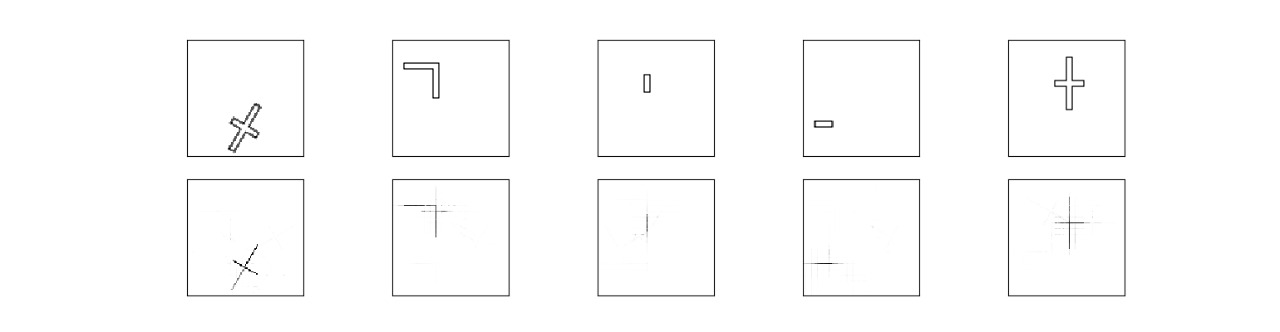
\includegraphics[width=\linewidth]{images/midcurvenn_simpleencoderdecoder}
	\captionof{figure}{Encoder Decoder network in Tensorflow/Keras} \cite{midcurvenngithub}
	\label{fig_simpleecd}
    \end{center}
    
\subsection{Text-to-Text  based Approach}
\label{subsec:7}    
    
\subsubsection{Prompt-based Approach}
\label{subsubsec:1} 
LLMs (Large Language Models), like GPT (Generative Pretrained Transformers), Llama, etc. can be employed to generate the midcurve. Idea is to give a prompt telling what needs to be done along with some examples, and see if LLMs can generate shape for the test example. Geometry has been serialized into text as a simple list of points \cite{kulkarni2023geometry}.

A few shots prompt developed:

\begin{lstlisting}[basicstyle=\tiny, breaklines=true, breakatwhitespace=true,label=lst:python]
You are a geometric transformation program that transforms input 2D polygonal profile to output 1D polyline profile. 
Input 2D polygonal profile is defined by set of connected lines with the format as:
input : [line_1, line_2, line_3,....] where lines are defined by two points, where each point is defined by x and y coordinates. So
line_1 is defined as ((x_1, y_1), (x_2,y_2)) and similarly the other lines.
Output is also defined similar to the input as a set of connected lines where lines are defined by two points, where each point is defined by x and y coordinates. So,
output : [line_1, line_2, line_3,....]

Below are some example transformations, specified as pairs of 'input' and the corresponding 'output'. After learning from these examples, predict the 'output' of the last 'input' specified.
Do not write code or explain the logic but just give the list of lines with point coordinates as specified for the 'output' format.

input:[((5.0,5.0), (10.0,5.0)), ((10.0,5.0), (10.0,30.0)), ((10.0,30.0), (35.0,30.0)), ((35.0,30.0), (35.0, 35.0)), ((35.0, 35.0), (5.0,35.0)), ((5.0,35.0), (5.0,5.0))]
output: [((7.5,5.0), (7.5, 32.5)), ((7.5, 32.5), (35.0, 32.5)), ((35.0, 32.5) (7.5, 32.5))]

input: [((5,5), (10, 5)), ((10, 5), (10, 20)), ((10, 20), (5, 20)), ((5, 20),(5,5))]
output: [((7.5, 5), (7.5, 20))]

input: [((0,25.0), (10.0,25.0)), ((10.0,25.0),(10.0, 45.0)), ((10.0, 45.0),(15.0,45.0)), ((15.0,45.0), (15.0,25.0)), ((15.0,25.0),(25.0,25.0)), ((25.0,25.0),(25.0,20.0)), ((25.0,20.0),(15.0,20.0)), ((15.0,20.0),(15.0,0)), ((15.0,0),(10.0,0)), ((10.0,0),(10.0,20.0)), ((10.0,20.0),(0,20.0)), ((0,20.0),(0,25.0))]
output: [((12.5,0), (12.5, 22.5)), ((12.5, 22.5),(12.5,45.0)), ((12.5, 22.5), (0,22.5)), ((12.5, 22.5), (25.0,22.5))]

input:[((0, 25.0), (25.0,25.0)),((25.0,25.0),(25.0,20.0)), ((25.0,20.0),(15.0, 20.0)), ((15.0, 20.0),(15.0,0)), ((15.0,0),(10.0,0)), ((10.0,0),(10.0,20.0)), ((10.0,20.0),(0,20.0)), ((0,20.0),(0, 25.0))]
output:
\end{lstlisting}

The first input example above represents an ‘L’ shape (shown \ref{fig_L}) and the second is an ‘I’, whereas the 3rd is a ‘Plus’ sign shape.

    \begin{center}
	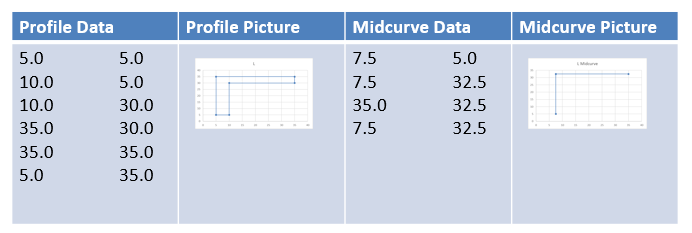
\includegraphics[width=0.8\linewidth]{images/L}
	\label{fig_L}
    \end{center}
    
    
The last shape for which LLM has been asked for the answer is actually a ‘T’ shape \ref{fig_T}. The picture below shows the correct/actual answer as well.

    \begin{center}
	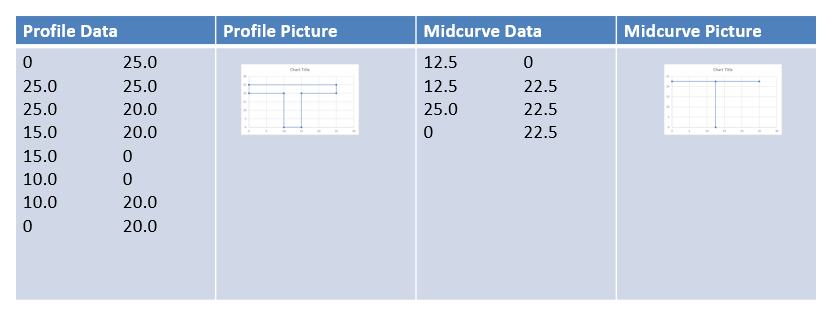
\includegraphics[width=0.8\linewidth]{images/T}
	\label{fig_T}
    \end{center}
    
And the outputs computed by various LLMs (ChatGPT, Perplexity AI, Bard) , along with the real/actual answer:

\begin{lstlisting}[basicstyle=\tiny, breaklines=true, breakatwhitespace=true, label=lst:python]
Actual: [((12.5,0), (12.5,22.5)), ((12.5,22.5),(25.0,22.5)), ((12.5,22.5),(0,22.5))]
ChatGPT: [((2.5, 0), (2.5, 22.5)), ((2.5, 22.5), (2.5, 45.0)), ((2.5, 22.5), (25.0, 22.5)), ((2.5, 22.5), (12.5, 22.5)), ((2.5, 22.5), (0, 22.5)), ((2.5, 22.5), (25.0, 22.5))]
Perplexity: [((12.5,0), (12.5, 22.5)), ((12.5, 22.5),(12.5,45.0)), ((12.5, 22.5), (0,22.5)), ((12.5, 22.5), (25.0,22.5))]
Bard: [((12.5, 0), (12.5, 25.0)), ((12.5, 25.0), (25.0, 25.0)), ((25.0, 25.0), (25.0, 0))]
\end{lstlisting}

Visually here is how results from different LLMs look:

    \begin{center}
	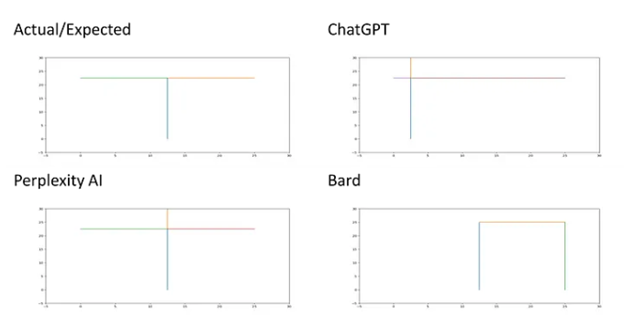
\includegraphics[width=0.8\linewidth]{images/actual_predicted}
	\label{fig_results}
    \end{center}
    
All of the above have failed. Even for the latest run on Oct 2023), the results are:
	\begin{itemize}
	\item {\bf llama 7B g4\_0 ggml}: \lstinline[basicstyle=\tiny, breaklines=true, breakatwhitespace=true]| (8, 17) & (64, 32)|: Wrong.
	\item {\bf Bard}: \lstinline[basicstyle=\tiny, breaklines=true, breakatwhitespace=true]|[((8.33,5),(8.33, 22.5)), ((8.33, 22.5), (25,22.5)), ((8.33, 22.5), (0,25))]|: Wrong.
	\item {\bf Hugging Chat}:  \lstinline[basicstyle=\tiny, breaklines=true, breakatwhitespace=true]|[((12.5, 0), (12.5, 22.5)), ((12.5, 22.5), (25.0, 22.5)), ((25.0, 22.5), (25.0, 25.0))]|: a bit wrong on the last line.
	\item {\bf GPT 4}:  \lstinline[basicstyle=\tiny, breaklines=true, breakatwhitespace=true]|[((12.5,0), (12.5,22.5)), ((12.5,22.5),(0,22.5)), ((12.5,22.5),(25.0,22.5))]| just change in sequence of lines, and that's inconsequential, so the answer is correct.
	\item {\bf Claude}:  \lstinline[basicstyle=\tiny, breaklines=true, breakatwhitespace=true]|[((12.5, 0.0), (12.5, 22.5)), ((12.5, 22.5), (12.5, 25.0)), ((12.5, 22.5), (0.0, 22.5)), ((12.5, 22.5), (25.0, 22.5))]|
\end{itemize}		    
    
Although other proprietary and open-source models need to catch-up with GPT-4, even GPT-4 needs to be developed further to understand not just sequential lines but graphs/networks with different shapes, essentially, the geometry.

\subsubsection{Fine-tuning based approach}
\label{subsubsec:2} 

One limitation of 2D geometry-shape, represented as a sequential list of points, is that we can not represent line intersections or concentric loops. To address this a more comprehensive structure has been proposed which is based on the corresponding 3D structure popular in Solid Modeling, called B-rep (Boundary Representation).

\begin{lstlisting}[basicstyle=\tiny, breaklines=true, breakatwhitespace=true, label=lst:python]
{
'ShapeName': 'I',
'Profile': [(5.0, 5.0), (10.0, 5.0), (10.0, 20.0), (5.0, 20.0)],
'Midcurve': [(7.5, 5.0), (7.5, 20.0)],
'Profile_brep': {
			'Points': [(5.0, 5.0), (10.0, 5.0), (10.0, 20.0),(5.0, 20.0)], # list of (x,y) coordinates
			'Lines': [[0, 1], [1, 2], [2, 3], [3, 0]], # list of point ids (ie index in the Points list)
			'Segments': [[0, 1, 2, 3]] # list of line ids (ie index in Lines list)
			},
'Midcurve_brep': {
			'Points': [(7.5, 5.0), (7.5, 20.0)],
			'Lines': [[0, 1]],
			'Segments': [[0]]
			},				
}
\end{lstlisting}

         \begin{center}
	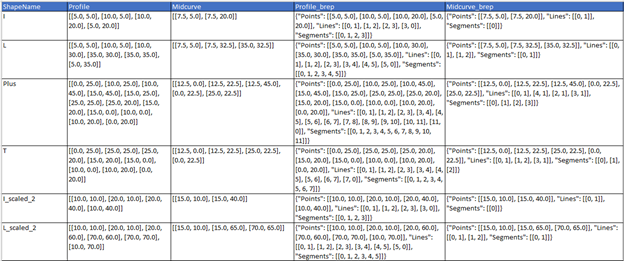
\includegraphics[width=\linewidth]{images/shapes_csv}
	\label{fig_csv}
    \end{center}

Column information is as below:
	\begin{itemize}
	\item {\bf ShapeName} (text): name of the shape. Just for visualization/reports.
	\item {\bf Profile} (text): List of Points coordinates (x,y) representing outer profile shape, typically closed.
	\item {\bf Midcurve} (text): List of Points coordinates (x,y) representing inner midcurve shape, typically open.
	\item {\bf Profile\_brep} (text): Dictionary in B-rep format representing outer profile shape, typically closed.
	\item {\bf Midcurve\_brep} (text): Dictionary in B-rep format representing inner midcurve shape, typically open.
	\end{itemize}

Each Segment is a continuous list of lines. In case of, say `Midcurve-T`, as there is an intersection, we can treat each line in a separate segment. In the case of 'Profile O', there will be two segments, one for outer lines and another for inner lines. Each line is a list of points, for now, linear. Points is a list of coordinates $(x,y)$, later can be $(x,y,z)$.

Once we have this Brep representations of both, profile and the corresponding midcurve, in the text form, then we can try various machine translation approaches or LLM based fine tuning or few-shots prompt engineering.

One major advantage of text based method over image based method is that image output still has stray pixels, cleaning which will be a complex task. But the text method has exact points. It may just give odd lines, which can be removed easily.

Dataset when imported looks like

%         \begin{center}
%	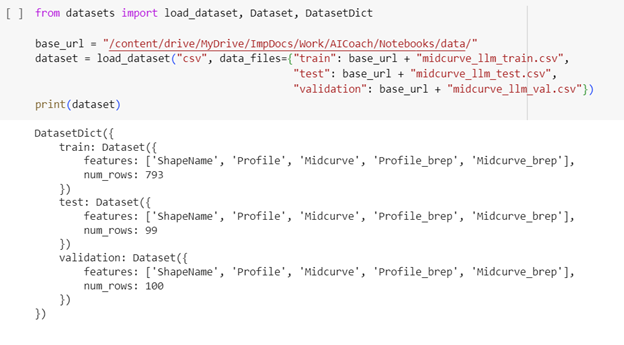
\includegraphics[width=\linewidth]{images/kaggle1}
%	\label{fig_k1}
%    \end{center}

\begin{lstlisting}[basicstyle=\tiny, breaklines=true, breakatwhitespace=true,label=lst:python]
from datasets import load_dataset, Dataset, DatasetDict

base_url = "/content/drive/MyDrive/ImpDocs/Work/AICoach/Notebooks/data/"
dataset = load_dataset("csv", data_files={"train": base_url + "midcurve_llm_train.csv",
                                          "test": base_url + "midcurve_llm_test.csv",
                                          "validation": base_url + "midcurve_llm_val.csv"})
DatasetDict({
    train: Dataset({
        features: ['ShapeName', 'Profile', 'Midcurve', 'Profile_brep', 'Midcurve_brep'],
        num_rows: 793
    })
    test: Dataset({
        features: ['ShapeName', 'Profile', 'Midcurve', 'Profile_brep', 'Midcurve_brep'],
        num_rows: 99
    })
    validation: Dataset({
        features: ['ShapeName', 'Profile', 'Midcurve', 'Profile_brep', 'Midcurve_brep'],
        num_rows: 100
    })
})

\end{lstlisting}

Preprocessing is done to tokenize, generate ids and prepare attention.

%         \begin{center}
%	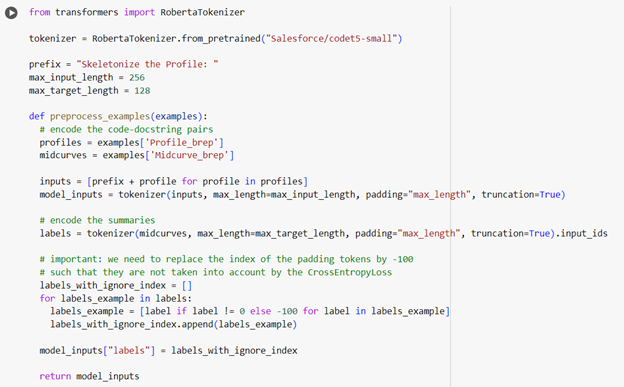
\includegraphics[width=\linewidth]{images/kaggle2}
%	\label{fig_k2}
%    \end{center}
%    

The dataset is used to fine-tune the base model called ``Salesforce/codet5-small''. Trained model is saved and used for inference on test samples.

\begin{lstlisting}[basicstyle=\tiny, breaklines=true, breakatwhitespace=true,label=lst:python]
from transformers import T5ForConditionalGeneration, AdamW, get_linear_schedule_with_warmup
import pytorch_lightning as pl

class CodeT5(pl.LightningModule):
    def __init__(self, lr=5e-5, num_train_epochs=15, warmup_steps=1000):
        super().__init__()
        self.model_name = "Salesforce/codet5-small"
        self.model = T5ForConditionalGeneration.from_pretrained(self.model_name)
        self.save_hyperparameters()
        
    def forward(self, input_ids, attention_mask, labels=None):
        outputs = self.model(input_ids=input_ids, attention_mask=attention_mask, labels=labels)
        return outputs        
        :
        :

model = CodeT5()

trainer = Trainer(max_epochs=5,accelerator="auto",# gpus=1,
                  default_root_dir="/content/drive/MyDrive/CodeT5/Notebooks/Checkpoints",
                  logger=wandb_logger,
                  callbacks=[early_stop_callback, lr_monitor])
trainer.fit(model)
\end{lstlisting}

%         \begin{center}
%	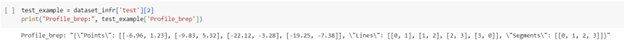
\includegraphics[width=\linewidth]{images/kaggle3}
%	\label{fig_k3}
%    \end{center}
%    
%         \begin{center}
%	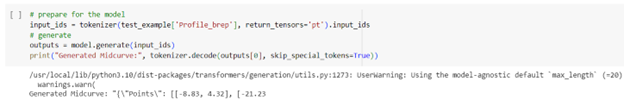
\includegraphics[width=\linewidth]{images/kaggle4}
%	\label{fig_k4}
%    \end{center}    
    
The output predicted far away from the corresponding ground truth. 

\begin{lstlisting}[basicstyle=\tiny, breaklines=true, breakatwhitespace=true,label=lst:python]
input_ids = tokenizer(test_example['Profile_brep'], return_tensors='pt').input_ids
outputs = model.generate(input_ids)

print("Ground truth:", test_example['Midcurve_brep'])
print("Generated Midcurve:", tokenizer.decode(outputs[0], skip_special_tokens=True))

Ground truth: "{\"Points\": [[-8.4, 3.28], [-20.68, -5.33]], \"Lines\": [[0, 1]], \"Segments\": [[0]]}"
Generated Midcurve: "{\"Points\": [[-8.83, 4.32], [-21.23
\end{lstlisting}

%         \begin{center}
%	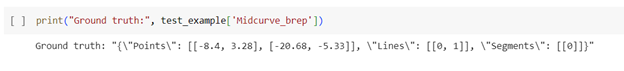
\includegraphics[width=\linewidth]{images/kaggle5}
%	\label{fig_k5}
%    \end{center}
    
There could be many reasons for the mismatch such as the quality of LLM, training parameters, and above all, need for a far bigger dataset for fine-tuning. But overall, the approach and priliminary results look promising to warrant further investigations.


\section{Conclusions}
\label{sec:5}

This research significantly advances midcurve computation by exploring the interplay between established methodologies and cutting-edge approaches, particularly integrating Large Language Models (LLMs). Emphasizing the nuanced nature of geometric dimension reduction, it identifies challenges in handling variable-length input data, representing intricate shapes, and addressing limitations in existing models.

 The MidcurveLLM with an Encoder-Decoder architecture and B-rep structures showcases promise, despite discrepancies with ground truths, pointing to the need for more extensive datasets and refined training parameters. Overall, this study serves as a crucial catalyst for advancing midcurve computation methodologies, inviting further scrutiny and advancements in the transformative intersection of geometry and advanced machine learning.


%This research not only contributes significantly to our understanding of midcurve computation but also illuminates the complex challenges and exciting potential avenues for future exploration. The study highlights the intricate interplay between established methodologies and cutting-edge approaches, particularly the integration of Large Language Models (LLMs) in midcurve generation. This underscores the nuanced nature of geometric dimension reduction and the need for innovative solutions to address the associated complexities.
%
%The work clearly delineates the challenges inherent in variable-length input data, the representation of intricate shapes, and the limitations of existing models like Seq2Seq and Image2Image networks. These limitations necessitate a paradigm shift towards more advanced and adaptable methodologies.
%The proposed MidcurveNN, utilizing an Encoder-Decoder architecture with supervised learning, demonstrates a promising direction for overcoming the hurdles plaguing traditional midcurve computation methods. The innovative application of Brep structures in fine-tuning LLMs represents a commendable effort towards achieving higher geometric precision in the generated midcurves.
%
%However, the observed discrepancies between the predicted outputs and ground truths highlight the need for more extensive datasets and further refinement of the training parameters. This ongoing research underscores the crucial role of extensive training data and meticulous fine-tuning in achieving optimal performance with LLM-based approaches.

In essence, this research serves as a vital catalyst for the advancement of midcurve computation methodologies. The seamless integration of LLMs, the exploration of novel geometric representations, and the introspection into fine-tuning mechanisms collectively contribute to the ongoing dialogue in geometric dimension reduction. 



%%%%%%%%%%%%%%%%%%%%%%%%%%%%%%%%%

\bibliographystyle{IEEEtran}
\bibliography{references}

\end{document}
